% 建议使用 XeLaTeX 或 LuaLaTeX 编译(中文与公式支持更佳)
\documentclass[UTF8,zihao=-4]{ctexart}

\usepackage[a4paper,margin=2.5cm]{geometry}
\usepackage{amsmath, amssymb, amsthm}
\usepackage{bm}
\usepackage{hyperref}
\usepackage{graphicx}
\usepackage{caption}
\usepackage{listings}
\usepackage{xcolor}
\usepackage{float}
\usepackage{placeins}
\graphicspath{{figures/}}

\lstdefinestyle{code}{
  basicstyle=\ttfamily\small,
  numbers=left,
  numberstyle=\tiny,
  numbersep=8pt,
  keywordstyle=\color{blue},
  commentstyle=\color{teal!70!black},
  stringstyle=\color{orange!70!black},
  showstringspaces=false,
  breaklines=true,
  frame=single,
  framerule=0.3pt,
  rulecolor=\color{black!15}
}
\lstset{style=code}

\title{K-means:原理、公式、应用与实战}
\author{}
\date{\today}

\begin{document}
\maketitle

\section{引言}
K-means 聚类通过最小化簇内平方和(within-cluster sum of squares, WCSS)来将数据划分为 \(K\) 个互不重叠的簇。算法交替执行“分配—更新”两步:先将样本分配给最近的质心,再以簇内样本均值更新质心。由于 K-means 默认簇形近似球形且密度相近,因此在标准化后的数值特征上表现最佳,对拉长或不规则簇需谨慎使用。

\section{原理与公式}
\subsection{目标函数}
设数据矩阵 \(\mathbf{X} = [\mathbf{x}_1,\dots,\mathbf{x}_n]^\top\),K-means 的优化目标为
\begin{equation}
\min_{\{C_k\},\{\bm{\mu}_k\}} \sum_{k=1}^K \sum_{\mathbf{x}_i \in C_k} \lVert \mathbf{x}_i - \bm{\mu}_k \rVert_2^2,
\end{equation}
其中 \(C_k\) 为第 \(k\) 个簇的样本集合,\(\bm{\mu}_k\) 为对应质心。最小化簇内方差等价于在总方差固定时最大化簇间方差。

\subsection{Lloyd 迭代}
常用的 Lloyd 算法流程如下:
\begin{enumerate}
  \item \textbf{初始化}:选择 \(K\) 个初始质心,推荐使用 k-means++ 以提升分散度。
  \item \textbf{分配}:基于所选距离度量(通常为欧氏距离)将每个样本指派到最近质心所在簇。
  \item \textbf{更新}:对每个簇重新计算质心,即簇内样本的均值。
  \item 循环执行分配和更新,直至质心移动量低于阈值或样本分配不再变化。
\end{enumerate}
算法一定收敛,但可能停留在局部最优;因此通常需要多次不同随机种子的重启。

\subsection{方差分解视角}
对标准化后的数据,总散度 \(\mathbf{S}_T\) 可写为簇内散度 \(\mathbf{S}_W\) 与簇间散度 \(\mathbf{S}_B\) 之和:\(\mathbf{S}_T = \mathbf{S}_W + \mathbf{S}_B\)。K-means 在迭代中持续降低 \(\text{tr}(\mathbf{S}_W)\),等价于提升簇间质心的分离度。

\section{应用与技巧}
\begin{itemize}
  \item \textbf{客户分群}:根据购买或行为特征对客户细分,以制定差异化运营策略。
  \item \textbf{向量量化}:在图像压缩、语音编码中用有限个原型向量近似原始样本。
  \item \textbf{特征工程}:将簇标签作为新的离散特征供后续监督学习模型使用。
  \item \textbf{实用建议}:对特征进行缩放,结合惯性与轮廓系数评估模型,并关注离群点的影响。
\end{itemize}

\section{Python 实战}
脚本 \texttt{gen\_clustering\_k\_means\_figures.py} 构造三个高斯簇并运行 K-means,同时绘制簇结果及惯性随簇数变化的肘部曲线。
\begin{lstlisting}[language=Python,caption={脚本 gen_clustering_k_means_figures.py 片段}]
from sklearn.cluster import KMeans

kmeans = KMeans(n_clusters=3, init="k-means++", n_init=10, max_iter=300,
                random_state=42)
labels = kmeans.fit_predict(points)

inertias = []
for k in range(1, 9):
    model = KMeans(n_clusters=k, init="k-means++", n_init=10,
                   max_iter=300, random_state=42)
    model.fit(points)
    inertias.append(model.inertia_)
\end{lstlisting}

\section{实验结果}
\begin{figure}[H]
  \centering
  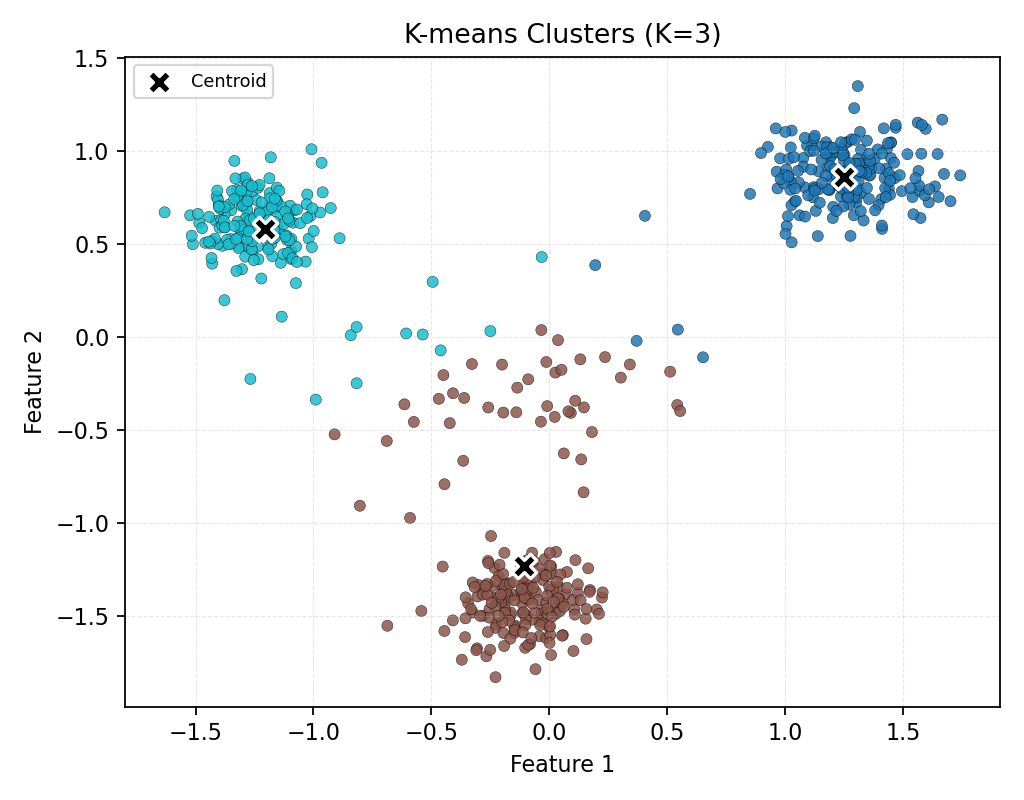
\includegraphics[width=0.82\linewidth]{kmeans_clusters.png}
  \caption{K-means 在合成高斯簇上的聚类结果(\(K=3\))}
  \label{fig:kmeans_clusters_cn}
\end{figure}

\begin{figure}[H]
  \centering
  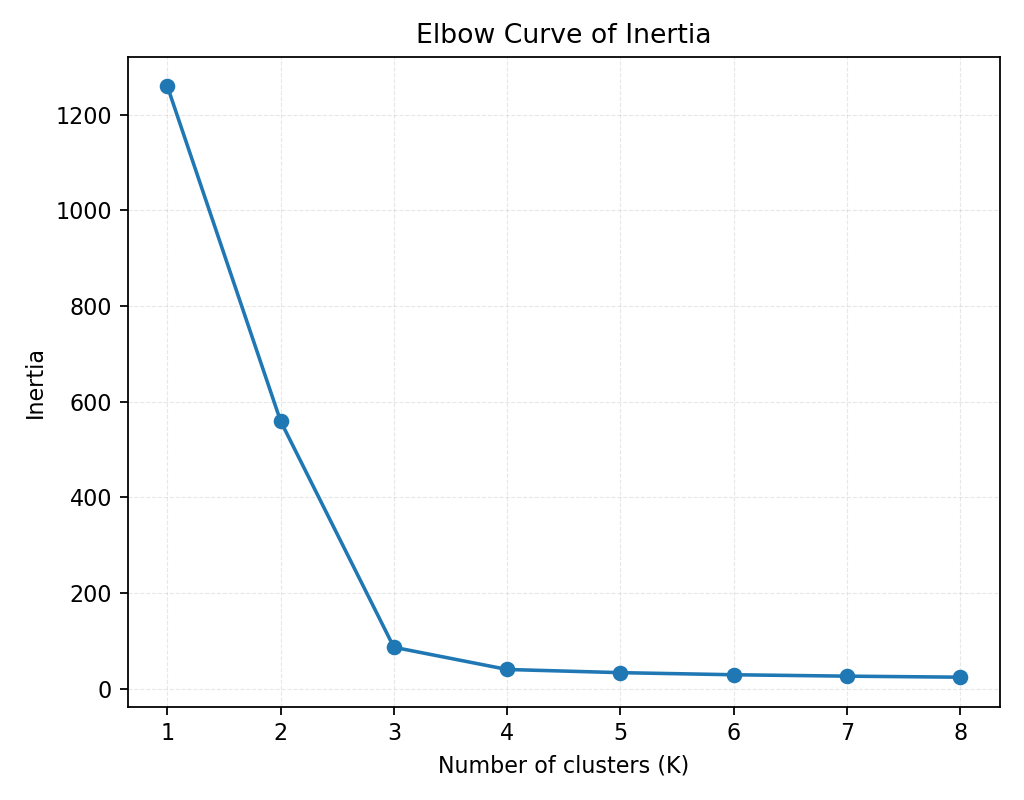
\includegraphics[width=0.82\linewidth]{kmeans_elbow.png}
  \caption{惯性与簇数的肘部曲线}
  \label{fig:kmeans_elbow_cn}
\end{figure}

\FloatBarrier
\section{总结}
K-means 以高效简洁著称,适合处理标准化的数值数据,并在簇呈球形且规模相近时表现稳定。合理的初始化、充分的重启次数以及肘部曲线等诊断工具有助于避免局部最优或过度划分。以上示例展示了从聚类结果到惯性分析的典型流程。

\end{document}
